\chapter{Objetivos}
\label{cap:capitulo3}

\begin{flushright}
\begin{minipage}[]{10cm}
\emph{Establecer metas es el primer paso para convertir lo invisible en visible.}\\
\end{minipage}\\

Tony Robbins\\
\end{flushright}

\vspace{1cm}

Escribe aquí un párrafo explicando brevemente lo que vas a contar en este capítulo. En este capítulo lo ideal es explicar cuáles han sido los objetivos que te has fijado conseguir con tu trabajo, qué requisitos ha de respetar el resultado final, y cómo lo has llevado a cabo; esto es, cuál ha sido tu plan de trabajo.\\

\section{Descripción del problema}
\label{sec:descripcion}

Cuenta aquí el objetivo u objetivos generales y, a continuación, concrétalos mediante objetivos específicos.

\section{Requisitos}
\label{sec:requisitos}

Describe los requisitos que ha de cumplir tu trabajo.

\section{Competencias}

Las competencias son aquellas habilidades, conocimientos y aptitudes que una persona emplea y adquiere para la realización, en este caso, del presente proyecto aunque es aplicable para cualquier tarea.
   
\subsection{Competencias empleadas}
Las competencias empleadas para la realización del presente proyecto fin de grado, que han sido tomadas de las distintas asignaturas del grado, son las siguientes: 

\begin{enumerate}
	\item{Evolución y futuro de la robótica: \textit{CE1.} Capacidad para analizar la evolución de la Ingeniería Robótica y ser capaz de identificar sus aplicaciones, oportunidades de emprendimiento y su impacto en el futuro. 
	Esta competencia ha sido empleada para poder desarrollar los capítulos 1 y 2 de este proyecto.}
	\item{Laboratorio de sistemas: \textit{CE9.} Capacidad de conocer y manejar los sistemas y las herramientas de las que dispone para su gestión y programación. 
	Esta competencia ha sido empleada para poder configurar y ejecutar código del robot en entornos no gráficos.}
	\item{Sensores y actuadores: \textit{CE12.} Capacidad de diseñar robots y sistemas inteligentes atendiendo a los elementos de sensorización y actuación más adecuados dependiendo de la aplicación, los requerimientos del sistema y las condiciones del entorno. 
	Esta competencia ha sido empleada para poder encontrar los componentes hardware necesarios para poder llevar a cabo el esqueleto del robot.}
	\item{Arquitectura \textit{software} para robots: \textit{CE15.} Capacidad de diseñar y programar aplicaciones robóticas y sitemas inteligentes en red usando \textit{middlewares}, mecanismos de comunicación y estándares propios del ámbito de la Ingeniería Robótica. 
	Esta competencia ha sido empleada en el momento de decidir el tipo de arquitectura \textit{software} necesaria a implementar en el robot.}
	\item{Visión artificial: \textit{CE25.} Capacidad de conocer y aplicar métodos de extracción de información a partir de la información percibida por cámaras y sensores 3D al desarrollo de aplicaciones en robots y sistemas inteligentes. 
	Esta competencia ha sido empleada para poder extraer información de la cámara y ser capaz de tratarla.}
	\item{Mecatrónica: \textit{CE32.} Capacidad de diseñar y construir robots móviles. Esta competencia ha sido empleada en el diseño e impresión en 3D de mi robot.}
	\item{Aprendizaje automático: \textit{CE27.} Capacidad de construir sistemas capaces de resolver problemas a partir de información no estructurada proporcionada por ejemplos o por la experiencia. 
	Esta competencia ha sido empleada para poder ser capaz de crear modelos de aprendizaje automático y aplicarlos al robot.}
\end{enumerate}

\subsection{Competencias adquiridas}

Las competencias adquiridas a lo largo del desarrollo del presente proyecto fin de grado que aparecen descritas en la guía docente de la propia asignatura, son las siguientes: 

\begin{enumerate}
	\item{\textit{CB2.} Que los estudiantes sepan aplicar sus conocimientos a su trabajo o vocación de una forma profesional y posean las competencias que suelen demostrarse por medio de la elaboración y defensa de argumentos y la resolución de problemas dentro de su área de estudio. 
	Esta competencia se adquiere gracias a la aplicación de las competencias empleadas justificadas anteriormente y que se pueden ver plasmadas en todo el proyecto.}
	\item{\textit{CB4.} Que los estudiantes puedan transmitir información, ideas, problemas y soluciones a un público tanto especializado como no especializado. 
	Esta competencia se aquiere al describir de forma precisa y comprensible todo el proceso complejo implicado en este proyecto dentro del presente documento.}
	\item{\textit{CB5.} Que los estudiantes hayan desarrollado aquellas habilidades de aprendizaje necesarias para emprender estudios posteriores con un alto grado de autonomía. 
	Esta competencia se logra al adquirir el conocimiento suficiente para desarrollar este trabajo de forma totalmente autónoma, contrastando información con distintas fuentes, haciendo pruebas con distintos tipos de \textit{software}, entre otras.}
	\item{\textit{CE28.} Desarrollo de las capacidades adecuadas para realizar un ejercicio original individual (o excepcionalmente colectivo), presentarlo y defenderlo ante un tribunal universitario, consistente en un proyecto en el ámbito de las tecnologías específicas del campo de la Robótica de naturaleza profesional en el que se sinteticen e integren las competencias adquiridas en las enseñanzas.
	Esta última competencia se cumple con el desarrollo de este proyecto: que abarca desde la elección del tema, el conocer el estado del arte, la implementación tanto hardware como software, el desarrollo de la presente memoria hasta su defensa ante un tribunal.}
\end{enumerate}


\section{Metodología}
\label{sec:metodologia}

Qué paradigma de desarrollo software has seguido para alcanzar tus objetivos.

\section{Plan de trabajo}
\label{sec:plantrabajo}

Qué agenda has seguido. Si has ido manteniendo reuniones semanales, cumplimentando objetivos parciales, si has ido afinando poco a poco un producto final completo, etc.




El presente proyecto trata ....\\


Después de aquí pasar al aparatado del estado del arte \\\\

En los textos puedes poner palabras en \textit{cursiva}, para aquellas expresiones en sentido \textit{figurado}, palabras como \textit{robota}, que está fuera del diccionario castellano, o bien para resaltar palabras de una colección: \textit{(a)} es la primera letra del abecedario, \textit{(b)} es la segunda, etc.\\

Al poner las dos líneas del anterior párrafo, este aparecerá separado del anterior. Si no las pongo, los párrafos aparecerán pegados. Sigue el criterio que consideres más oportuno.

\section{Segunda sección}
\label{sec:segundaseccion}

No olvides incluir imágenes y referenciarlas, como la Figura \ref{fig:roomba}.

\begin{figure} [h!]
	\begin{center}
		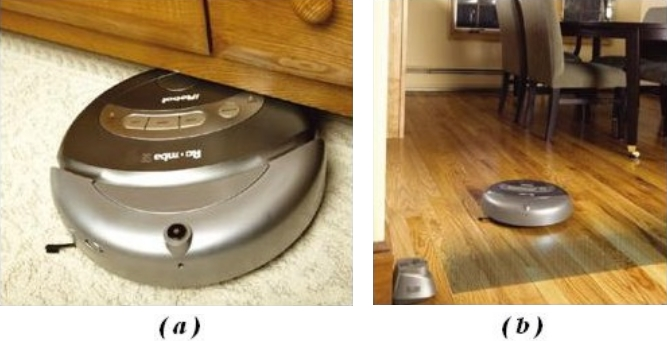
\includegraphics[width=8cm]{figs/roomba}
	\end{center}
	\caption{Robot aspirador Roomba de iRobot.}
	\label{fig:roomba}
\end{figure}\

Ni tampoco olvides de poner las URLs como notas al pie. Por ejemplo, si hablo de la Robocup\footnote{\url{http://www.robocup.org}}.

\subsection{Números}
\label{sec:subseccion}

En lugar de tener secciones interminables, como la Sección \ref{sec:robotica}, divídelas en subsecciones.

Para hablar de números, mételos en el entorno \textit{math} de \LaTeX, por ejemplo, $1.5Kg$. También puedes usar el símbolo del Euro como aquí: 1.500\euro.

\subsection{Listas}

Cuando describas una colección, usa \texttt{itemize} para ítems o \texttt{enumerate} para enumerados. Por ejemplo:

\begin{itemize}
	\item \textit{Entorno de simulación.} Hemos usado dos entornos de simulación: uno en 3D y otro en 2D.
	\item \textit{Entornos reales.} Dentro del campus, hemos realizado experimentos en Biblioteca y en el edificio de Gestión.
\end{itemize}\

\begin{enumerate}
	\item Primer elemento de la colección.
	\item Segundo elemento de la colección.
\end{enumerate}\

\paragraph{Referencias bibliográficas}
\label{sec:referencias}

Cita, sobre todo en este capítulo, referencias bibliográficas que respalden tu argumento. Para citarlas basta con poner la instrucción \verb|\cite| con el identificador de la cita. Por ejemplo: libros como \cite{vega12e}, artículos como \cite{vega19b}, URLs como \cite{vega19a}, tesis como \cite{vega18b}, congresos como \cite{vega18a}, u otros trabajos fin de grado como \cite{vega08b}.

Las referencias, con todo su contenido, están recogidas en el fichero \texttt{bibliografia.bib}. El contenido de estas referencias está en formato \texttt{BibTex}. Este formato se puede obtener en muchas ocasiones directamente, desde plataformas como \texttt{Google Scholar} u otros repositorios de recursos científicos.

Existen numerosos estilos para reflejar una referencia bibliográfica. El estilo establecido por defecto en este documento es APA, que es uno de los estilos más comunes, pero lo puedes modificar en el archivo \texttt{memoria.tex}; concretamente, cambiando el campo \verb|apalike| a otro en la instrucción \verb|\bibliographystyle{apalike}|. 

\

\

\

Y, para terminar este capítulo, resume brevemente qué vas a contar en los siguientes.
